\documentclass[letterpaper]{article}
\usepackage[utf8]{inputenc}
\usepackage[spanish]{babel}
\usepackage[letterpaper,includeheadfoot, top=.5cm, bottom=3.0cm, right=2.0cm, left=2.0cm]{geometry}
\renewcommand{\familydefault}{\sfdefault}
\usepackage{amsmath}
\usepackage{graphicx}
\usepackage{subcaption}
\usepackage{gensymb}
\usepackage{color}
\usepackage{hyperref}
\usepackage{amssymb}
\usepackage{url}
%\usepackage{pdfpages}
\usepackage{fancyhdr}
\usepackage{enumerate}
\usepackage{float}
\usepackage{tikz}
\usetikzlibrary{patterns}
\usepackage{siunitx}
\usepackage{framed}
\tikzset{
every picture/.append style={
  execute at begin picture={\deactivatequoting},
  execute at end picture={\activatequoting}
  }
}
%-------------------- CABECERA ---------------------
\pagestyle{fancy}
\fancyhf{}
\author{Martin Bataille}
\date{}
\title{\bf Torque}
%Encabezado
\fancyhead[R]{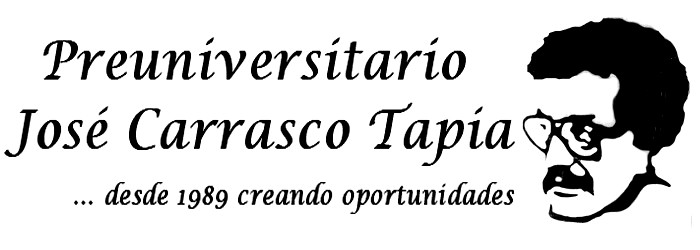
\includegraphics[scale=0.35]{jct.jpg}}
\fancyfoot[C]{\thepage}


\newcommand{\tpb}[1]{node[midway, below, sloped] {#1}}
\newcommand{\tpa}[1]{node[midway, above, sloped] {#1}}
\newcommand{\tvec}[3]{[->, thick] #1 -- #2 \tpb{#3}}
\newcommand{\tveca}[3]{[->, thick] #1 -- #2 \tpa{#3}}
\newcommand{\tvecnotsloped}[3]{[->, thick] #1 -- #2 {node[midway, above] {#3}}}

\newcounter{propiedades}
\newcounter{definiciones}

\newcommand{\propi}{\stepcounter{propiedades} \textbf{Propiedad \thepropiedades}: }
\newcommand{\defii}{\stepcounter{definiciones} \textbf{Definición \thedefiniciones}: }

\newenvironment{prop}
{ \begin{framed} \propi}
{ \end{framed} }
\newenvironment{defi}{\begin{framed} \defii}{\end{framed}}

\renewcommand{\sectionmark}[1]{\markright{\thesection.\ #1}}
\renewcommand{\headrulewidth}{0.5pt}
\renewcommand{\footrulewidth}{0pt}
\setlength{\headheight}{92pt}

% --------------- ---------PORTADA -----------------------
\begin{document}
\maketitle
\thispagestyle{fancy}
\begin{center}
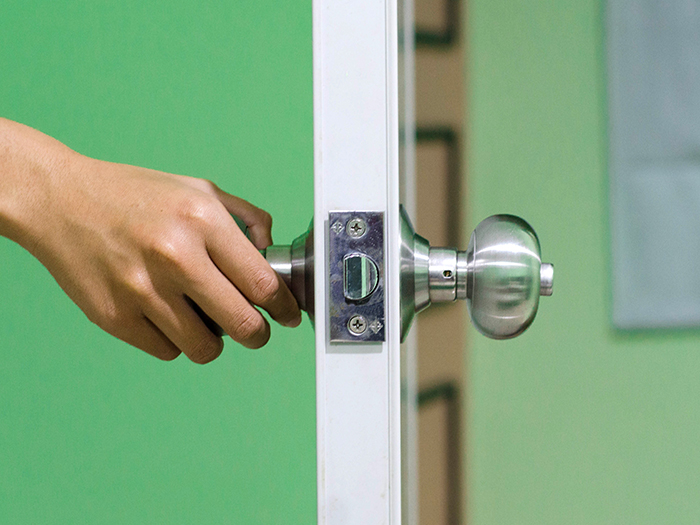
\includegraphics[scale=1.2]{portada.jpg}
\end{center}
\pagebreak

¿Por qué el pomo de la puerta está del lado opuesto a las bisagras? ¿Qué cambiaría si uno pone el pomo de la puerta del lado de las bisagras? ¿Por qué no se puede balancear un lápiz sobre su punta? Aunque estas preguntas puedan parecer muy estúpidas, la respuesta no es trivial. Todo esto y mucho más lo resolveremos al final de esta guía!

\section*{Introducción}

Hemos aprendido que las fuerzas provocan cambios en el movimiento de los objetos a través de $F = ma$. Sin embargo, esto solo explica la traslación de los objetos que constituye solo una parte del movimiento de los cuerpos. Un ejemplo se presenta cuando lanzamos una botella plástica esperando que caiga de verticalmente y quede estable, procediendo después a hacer un \emph{dab}. Ahí la botella no solo se traslada de nuestra mano hasta el piso (de lo contrario sería demasiado fácil y no se merecería un \emph{dab}), sino que también rota en el aire. Pero, ¿por qué se produce esa rotación?

Como veremos a lo largo de esta guía, esa rotación se debe a que ejercemos una fuerza sobre el cuerpo, esa fuerza provoca un torque en el cuerpo y el torque se traduce en movimiento rotacional.

\section*{¿Cómo se define el torque?}

Antes de definir el torque tenemos que entender unos conceptos primero. Al momento de abrir una puerta, uno puede comprobar experimentalmente dos cosas: 
\begin{itemize}

\item es más fácil abrirla mientras más lejos del eje de rotación (donde están las bisagras) la empujemos.

\item es más fácil abrirla mientras el ángulo entre la dirección de la fuerza y la puerta se acerca a \ang{90}.

\end{itemize}

Podemos entonces deducir que antes de definir el torque tenemos que definir esta distancia entre el eje de rotación y el punto donde se aplica la fuerza, y el ángulo. Para esto es muy útil pensar en el vector que va desde el eje de rotación hasta el punto donde se aplica la fuerza. A este vector se le llama brazo de palanca.

\begin{defi}
El brazo de palanca se suele escribir como $\vec{r}$ o $\vec{b}$ y representa el vector que va desde el eje de rotación hasta el punto donde se aplica la fuerza.
\end{defi}

Volviendo al ejemplo de la puerta, podemos pensar en el caso que aplicamos dos fuerzas en distintos puntos y con distinta dirección, como en la figura siguiente. El problema es, ¿qué fuerza permite abrir con mayor fácilidad la puerta? La respuesta está en el torque.

\begin{figure}[h]
\centering
\begin{tikzpicture}
\fill [pattern=north east lines] (0,0) rectangle (5,0.5);
\draw (0,0) rectangle (5,0.5);
\draw [->] (4.5,0) -- (6,2) node[midway, below, right] {$\vec{F}_2$};
%\draw (4.5,2.5) node[above] {$\vec{F}_2$};
\draw [->] (0,-0.6) -- (4.5,-0.6) node[midway, below] {$\vec{r}_2$}; 
\draw [->] (3.5,0) -- (3.5,2.5);
\draw (3.5,2.5) node[above] {$\vec{F}_1$};
\draw [->] (0, -0.1) -- (3.5, -0.1) node[midway, below] {$\vec{r}_1$};
\end{tikzpicture}
\end{figure}

\begin{defi}
El torque o momento de fuerza es un vector que se define como el producto cruz entre el brazo de palanca $\vec{r}$ y la fuerza aplicada $\vec{F}$,
$$\vec{\tau} = \vec{r}\times\vec{F}$$

Lo que es equivalente a,
$$|\vec{\tau}| = |\vec{r}|\cdot|\vec{F}|\cdot\cos{\theta}$$

Donde $\theta$ representa el ángulo que se forma entre la fuerza aplicada y el brazo de palanca, y la dirección de $\vec{\tau}$ está dada por la regla de la mano derecha.

Se deduce que la magnitud del torque se mide en \si{N.m}
\end{defi}

Volviendo al ejemplo de la puerta, tomemos $r_1 = 0.4\ \si{m}$, $F_1 = 10\ \si{N}$, $\theta_1 = \frac\pi2\ \si{rad}$, $r_2 = 0.8\ \si{m}$, $F_2 = 10\ \si{N}$ y $\theta_2 = \frac\pi3\ \si{rad}$, donde $\theta_2$ representa el ángulo entre $\vec{r}_2$ y $\vec{F}_2$. ¿Qué fuerza ejerce un mayor torque?

Primero, notemos que por la regla de la mano derecha, $\vec{\tau}_1$ y $\vec{\tau}_2$ tienen la misma dirección y sentido, basta entonces ver qué vector tiene mayor magnitud. Luego, aplicamos la definición de torque:
\begin{align*}
|\vec{\tau}_1| &= |\vec{r}_1|\cdot|\vec{F}_1|\cdot\cos{\theta_1} = 0.4 \cdot 10 \cdot \cos{\frac\pi2} = 4\ \si{N.m} \\
|\vec{\tau}_2| &= |\vec{r}_2|\cdot|\vec{F}_2|\cdot\cos{\theta_2} = 0.8 \cdot 10 \cdot \cos{\frac\pi3} = 8\cdot\frac12 = 4\ \si{N.m}
\end{align*}

Sorprendentemete, las dos fuerzas producen el mismo torque! ¿Pero qué significa eso respecto al movimiento de la puerta? Para responder a esta pregunta tenemos que introducir una relación muy importante para el estudio de la rotación de los objetos, la famosa segunda ley de Newton para la rotación:

\begin{prop}
El torque y la aceleración angular están íntimamente relacionados de manera análoga a la fuerza y la aceleración lineal:
$$\vec{\tau} = I\vec{\alpha}$$

Donde $I$ representa el momento de inercia de un cuerpo y $\vec{\alpha}$ su aceleración angular.
\end{prop}

\section*{¿Qué es el momento de inercia?}

Dicho simplemente, el momento de inercia es el equivalente de la masa para la rotación de los cuerpos. Cuando estudiamos fuerzas y dinámica vimos que la masa de un objeto es la capacidad que tiene para resistirse al cambio de su movimiento. En el caso de la rotación, es el momento de inercia y no la masa la que determina su resistencia al cambio de movimiento (rotacional). Un ejemplo sencillo es el de la escoba, mientras uno no rompa o separe la escoba en varias partes, su masa va a ser constante lo que implica que al aplicarle la misma fuerza, se va a mover lo mismo. En cambio, si uno quiere rotar la escoba, observará que es más fácil rotar la escoba en torno al eje que pasa por el centro del palo de la escoba. Si se intenta rotar la escoba respecto a un eje perpendicular al palo de la escoba será mucho más difícil. Esto se debe a que el momento de inercia de un cuerpo depende del eje respecto al cual se rota el cuerpo.

\begin{defi}
El momento de inercia de un cuerpo representa su capacidad de resistirse al movimiento de rotación y se determina en función de la repartición de la masa en torno al eje de rotación. Mientras la masa se concentre más cerca del eje de rotación, menor será su momento de inercia, por lo tanto, más fácil será hacerlo rotar. En cambio, si la masa se concentra lejos el eje de rotación, mayor será el momento de inercia y más difíci será hacerlo rotar.

Para un cuerpo puntual, su momento de inercia está dado por:
$$I = mr^2$$

Donde $m$ representa la masa del cuerpo y $r$ la distancia desde el cuerpo hasta el eje de rotación. Se deduce que la unidad del momento de inercia según el \emph{SI} es \si{kg.m^2}.
\end{defi}

Como el momento de inercia depende de la forma del objeto y de la posición del eje de rotación no es necesario conocer el valor asociado a cada forma, solo basta recordar que mientrás más lejos esté repartida la masa respecto al eje de rotación mayor será el momento de inercia. En la figura siguiente se puede apreciar el momento de inercia en el caso de algunas formas geométricas.

\begin{figure}[h]
\centering
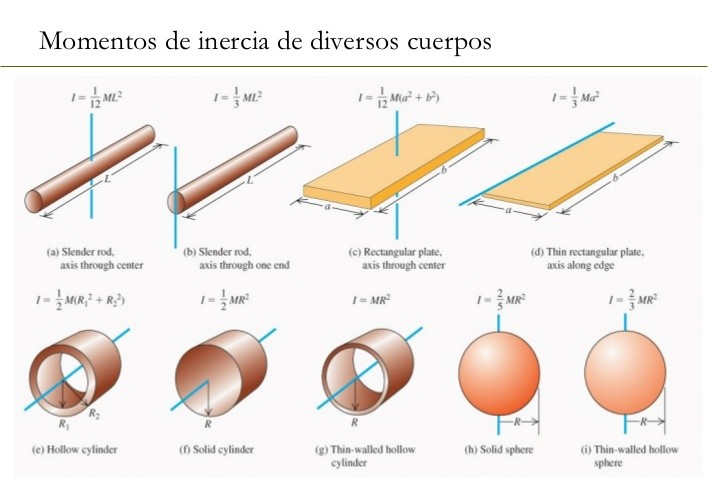
\includegraphics[scale=0.4]{momentos_de_inercia.jpg}
\end{figure}

\section*{Equilibrio estático}

Un problema recurrente en el estudio de fuerzas y rotación, son las condiciones para que un cuerpo esté estático. Se entiende que un cuerpo está estático cuando está y permanece en reposo. En otras palabras, su aceleración y su velocidad son nulas. De manera formal, para que un cuerpo esté completamente estático se tienen que cumplir cuatro condiciones:
\begin{itemize}
\item La velocidad lineal $v$ tiene que ser nula.
\item La fuerza neta sobre el objeto tiene que ser nula.
\item La velocidad angular $\omega$ tiene que ser nula.
\item El torque neto sobre el objeto tiene que ser nulo.
\end{itemize}

Es importante notar que incluso si la fuerza neta sobre un cuerpo es nula, eso no implica que el torque neto sea nulo. Dos fuerzas de igual magnitud que tienen sentido opuesto pero se aplican en distintos puntos del cuerpo provocan un torque neto que no es nulo mientras que la fuerza neta sobre el cuerpo si es nula.



\section*{Ejercicios}

\begin{enumerate}

\item Pendiente

\end{enumerate}

\section*{Problemas}

\begin{enumerate}

\item Pendiente

\end{enumerate}

\end{document}